\newpage
\section{Introduction}
MetaDoc is created as a way to securely transport data between a server and 
sites. It is created to improve the flow of information between \gls{hpc} sites
and Uninett Sigma \cite{improvingflow}.

MetaDoc consists of a client, running at the site, and a server running at the
Metacenter. MetaDoc takes care of authenticating the client on the server,
packing and unpacking the data to and from \gls{xml}, and transporting the data
securely between client and server. 

\begin{figure}[h!]
    
\includegraphics[width=\textwidth]{img/get_data}
    \caption{Client requesting data from server}
    \label{fig:get_data}
\end{figure}

\begin{figure}[h!]
    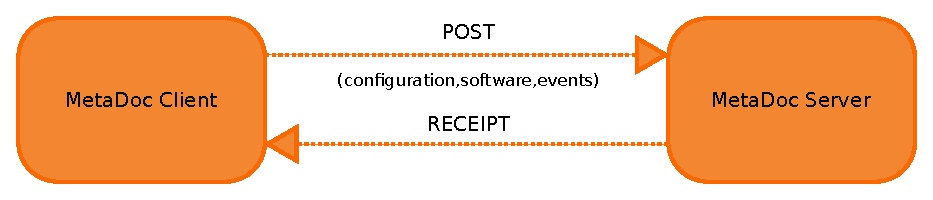
\includegraphics[width=\textwidth]{img/post_data}
    \caption{Client sending data to server. Server returns a receipt for
    recieved data.}
    \label{fig:post_data}
\end{figure}

In section \ref{sec:usage}, basic use of the MetaDoc client is explained. The
setup needed in order for the client to run, the availible handles and what the
client does itself is explained. If your goal is to get the client up and
running as quickly as possible, the MetaDoc Client Quick Start Guide is a good
place to start \cite{quick_start_guide}.

Section \ref{sec:server_api} goes through the server side API
